\documentclass[11pt,a4paper,twocolumn]{report}
\usepackage[utf8]{inputenc}
\usepackage[english]{babel}
\usepackage{amsmath}
\usepackage{amsfonts}
\usepackage{amssymb}
\usepackage{graphbox}
\usepackage{color}
\usepackage{listings}
\usepackage{hyperref}
\hypersetup{pdftex,colorlinks=true,allcolors=blue}
\usepackage{hypcap}
\usepackage[parfill]{parskip}
\usepackage{subcaption}
\usepackage{caption}
\usepackage{wrapfig}
\usepackage[rmargin=1.5cm, lmargin=1.5cm, bmargin=2cm, tmargin=2cm]{geometry}
\usepackage{verbatim}
\usepackage{xcolor}
\usepackage{circuitikz}
\usepackage{import}

\lstdefinestyle{Arduino}{%
    keywords={void},%                 define keywords
    keywordstyle=\bfseries\color{orange},
    identifierstyle=\color{orange},
    morecomment=[l]{//},%             treat // as comments
    morecomment=[s]{/*}{*/},%         define /* ... */ comments
    emph={HIGH, OUTPUT, LOW},%        keywords to emphasize
    emphstyle=\bfseries\color{blue},
}
\setlength{\columnsep}{1.2cm}
\begin{document}
\lstset{basicstyle = \ttfamily,columns=fullflexible}
\pagestyle{plain}
\newcommand{\HRule}{\rule{\linewidth}{0.5mm}}

\begin{titlepage}
\begin{center}
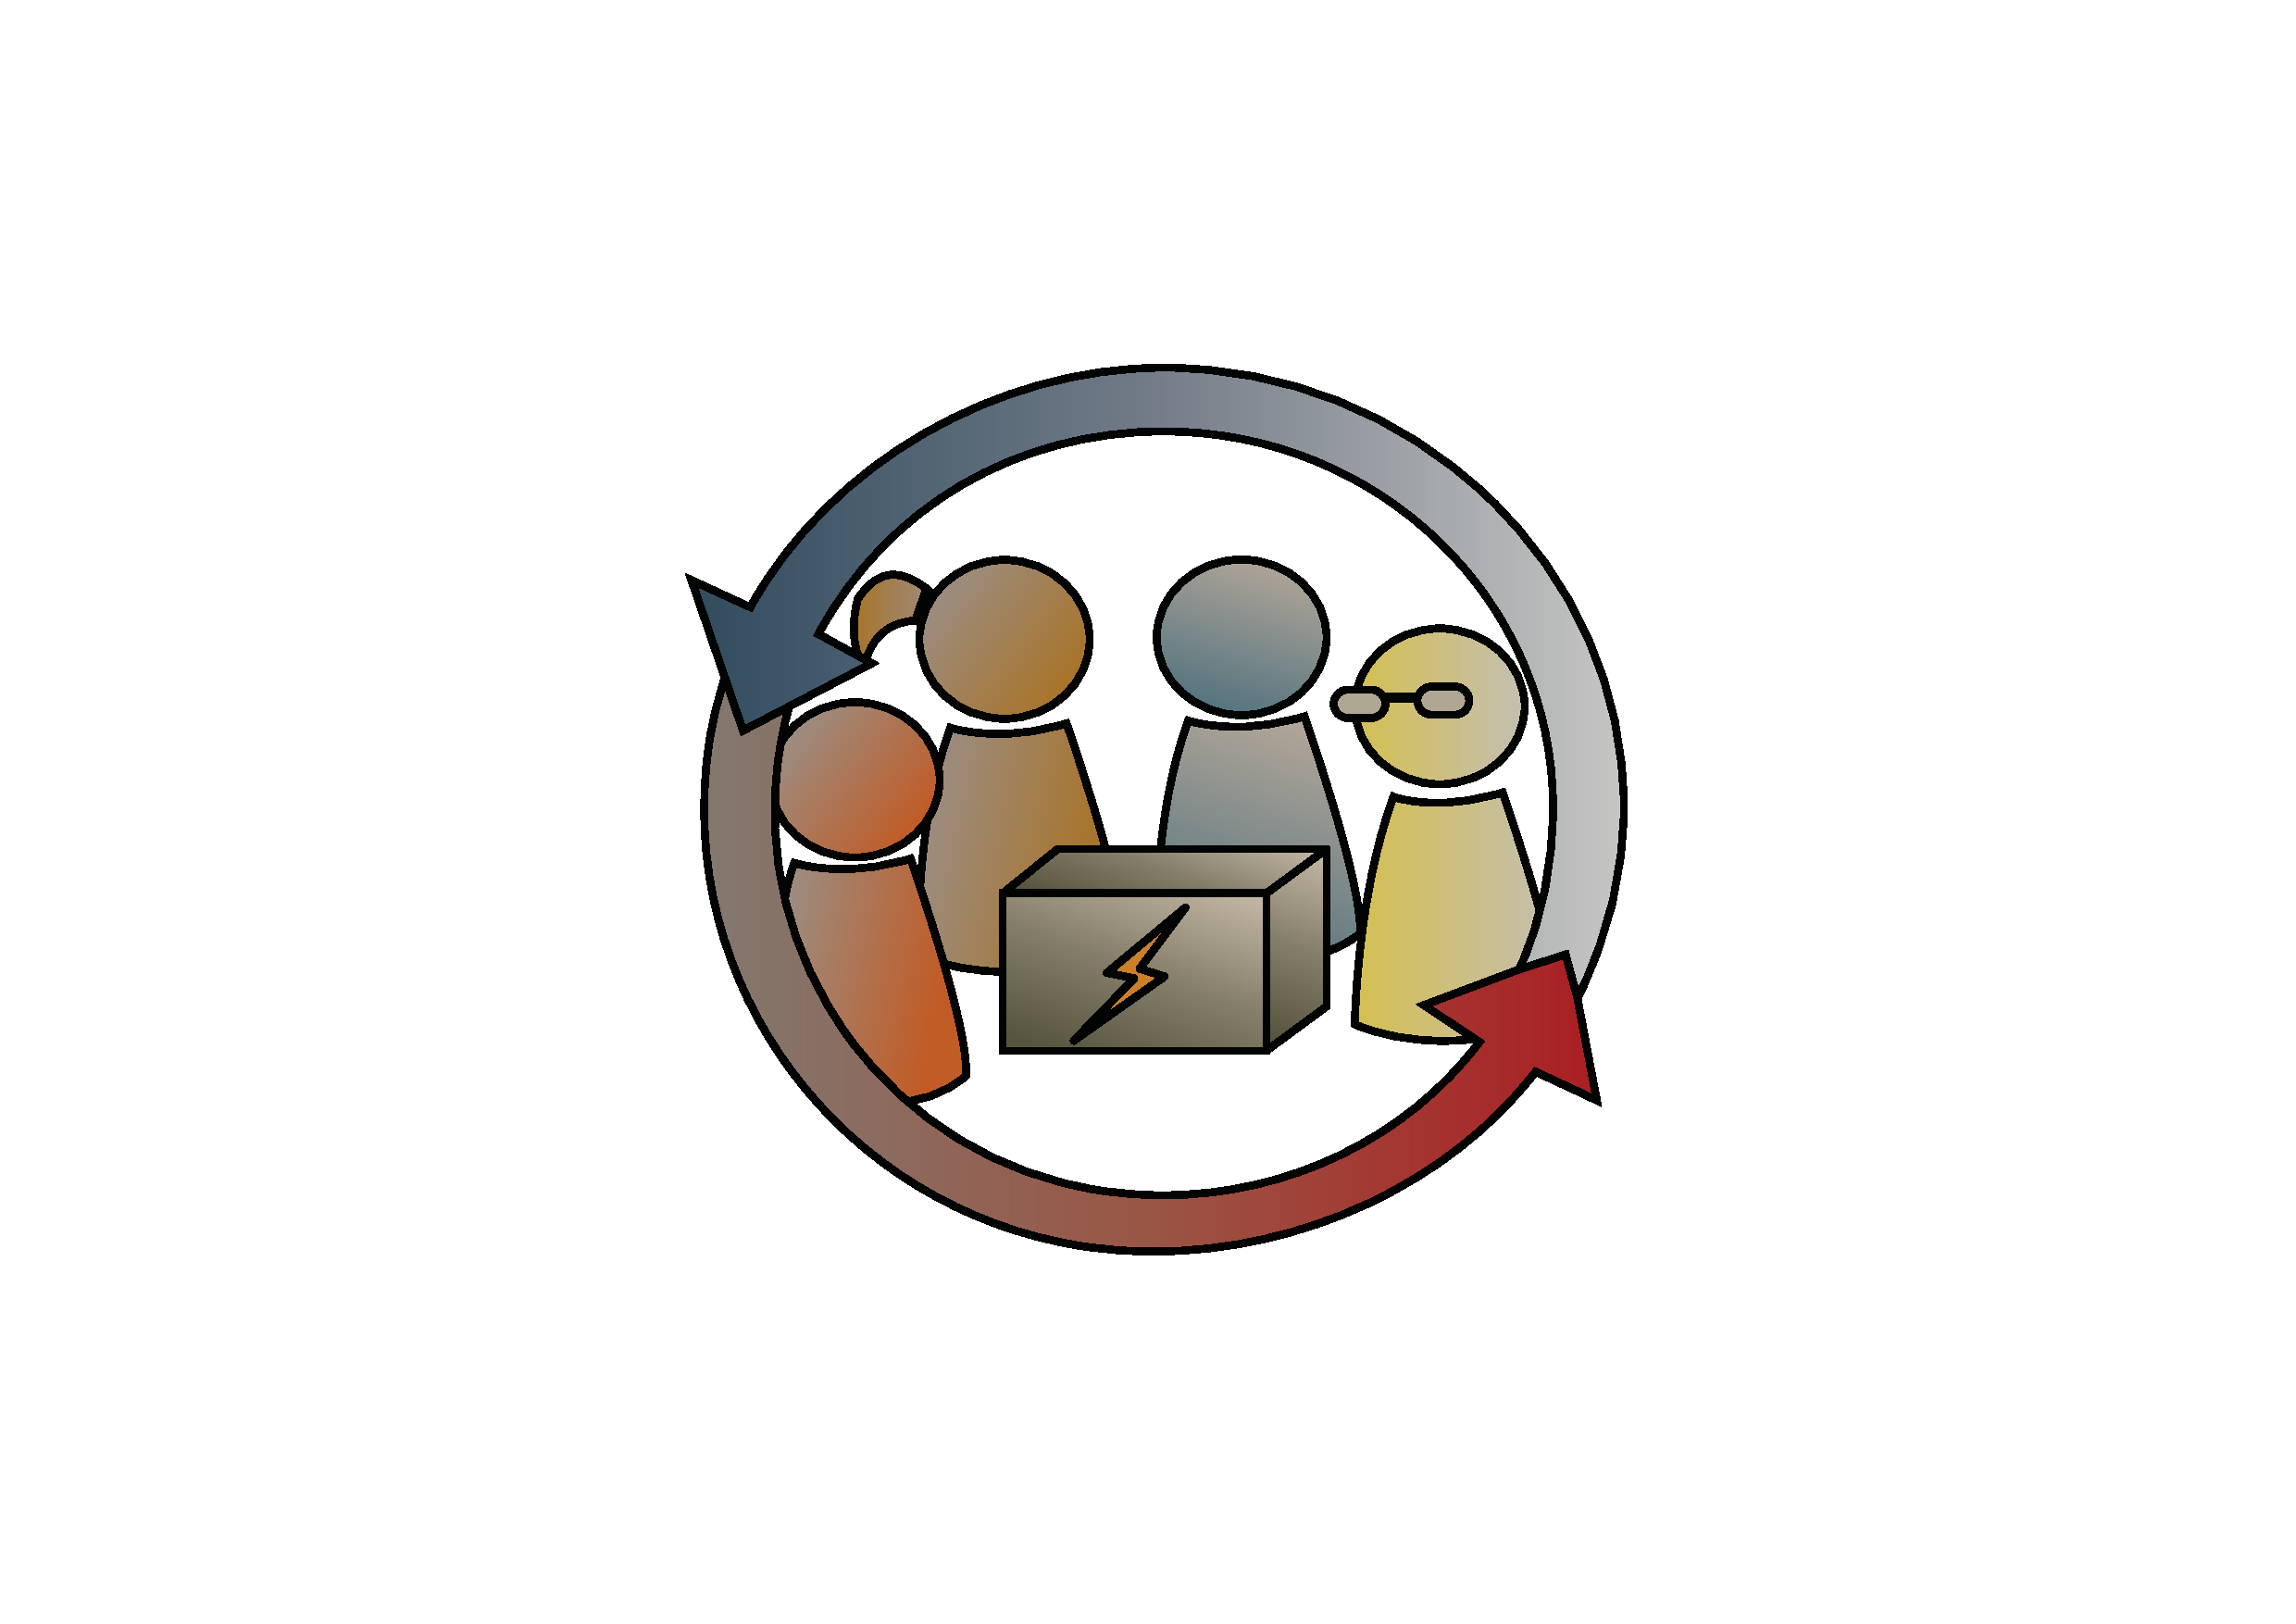
\includegraphics[width=0.75\textwidth]{./Misc/logo}~\\[1cm]

% Upper part of the page. The '~' is needed because \\
% only works if a paragraph has started.

\textsc{\LARGE Connected Community HackerSpace}\\[1.5cm]
% Title
\HRule \\[0.5cm]
{ \huge \bfseries Arduino Beginners Guide\\[0.5cm] }
\HRule \\[3.5cm]
\includegraphics[width=0.25\textwidth]{./Misc/arduino_logo}~
\vfill

% Bottom of the page
{\large \today}

\end{center}
\end{titlepage}

\tableofcontents
\subimport*{Chapter1/}{Chapter1.tex}
\subimport*{Appendix/}{Appendix.tex}

\end{document}
